\documentclass[a4paper,10pt]{article}
\usepackage[utf8x]{inputenc}
\usepackage{multirow}
\usepackage[pdftex]{graphicx}
\usepackage{float}
\usepackage[table]{xcolor}

% environment variables
\newenvironment{my_itemize}
{\begin{itemize}
  \setlength{\itemsep}{0cm}
  \setlength{\parskip}{0cm}}
{\end{itemize}}
\newenvironment{my_enumerate}
{\begin{enumerate}
  \setlength{\itemsep}{0cm}
  \setlength{\parskip}{0cm}}
{\end{enumerate}}

\newenvironment{my_description}
{\begin{description}
  \setlength{\itemsep}{0cm}
  \setlength{\parskip}{0cm}}
{\end{description}}


\begin{document}

\begin{titlepage}
\vspace{-1.5cm}
\begin{center}

\includegraphics[width=2cm]{Logo_Alexandria_University.jpg}\\
\vspace{1cm}
\textbf{\large ALEXANDRIA UNIVERSITY} \\
\textbf{FACULTY OF ENGINEERING} \\
{\small  COMPUTER AND SYSTEMS ENGINEERING DEPARTMENT}

\vspace{2.5cm}
\textbf{\LARGE Conceptualization Document}\\
\textbf{\small Smart Email Automatic Email Classification and Summarization}\\
{\small Inspired from TopCoder Direct Businees Requirements document}\\

\vspace{1cm}
{ Ahmed El-Sharkasy, Ahmed Kotb, Amr Nabil, Mohammad Kotb, Moustafa Mahmoud }
\end{center}

\vspace{1ex}
\textbf{Supervisors:} Prof. Dr. Mohamed Abou-gabal, Dr. Mustafa ElNainay
\end{titlepage}

\newpage
\tableofcontents
\newpage

\section{Introduction}

\subsection{Overview Application}
Email has become an efficient and popular communication mechanism as the number 
of Internet users increases. Therefore, email management has become an important 
and growing problem for individuals and organizations because it is prone to misuse.

One of the problems that are most important is disordered email messages, 
congested and unstructured emails in mail boxes. It may be very hard to 
find archived email messages, search for previous emails with specified contents 
or features when the mails are not well structured and organized. Also, email 
summarization is another important and challenging problem.

`Smart Email' is an application addressing these problems by providing automatic 
email summarization and categorization into folders.

%==============================================================================
\subsection{Project Objectives}
The business objectives of this project are listed below. Delivering these 
objectives will deliver the expected benefits of the application.
\begin{my_itemize}
  \item Automatically organizing congested and uncategorized emails into folders.
  \item Summarizing long email threads into a brief summary describing the 
	main points in these threads.
\end{my_itemize}


%==============================================================================
\subsection{Assumptions}
Some assumptions generally must be made in order to write a succinct definition 
of the application. Some assumptions are technical, while others are business natured.  Assumptions 
critical to the success of this project are listed below:
\begin{my_itemize}
  \item each user will have his own trained classification and summarization 
	models based on the user supplied training data;
  \item a web service will be implemented to provide email 
	classification and summarization support for different mail 
	servers (Example: Google, Hotmail, Yahoo);
  \item english language will be supported by default;
  \item email summarization will be provided as an on-demand service by the application user;
  \item the servers providing the web service have to provide sufficient 
	processing power for achieving reasonable response time;
  \item email classification will be based on the email subject and content. 
	Other features can be used as well, such as the email sender and recepient(s). 
	However, email attachments will not be considered as a classification feature for the email.
\end{my_itemize}

%==============================================================================
\subsection{Limitations}
Some limitations are assumptions on the extent of feature scope. Others are restrictions on resources 
or methods for achieving the objectives. The limitations of this project are listed below:

\begin{my_itemize}
  \item sufficient number of emails is needed for each email label to achieve 
	a reasonable classification accuracy;
  \item emails with size less than a specified threshold cannot be summarized.
\end{my_itemize}

%==============================================================================
\subsection{Open items and Risks}
During the conceptualization of the project and in the process of writing this document, 
some issues remain open.
\begin{my_itemize}
  \item Multi-label classification.
  \item Arabic support.
  \item The need for a client side application to assist the server side.
  \item Online training for classification models.
  \item Specifications for the web server providing the web service.
\end{my_itemize}


%==============================================================================
\newpage
\section{Proposed Workflow}
%==============================================================================
\subsection{Overview}
This section includes a concise description of the features and operation of the 
proposed solution. The context and workflow of the proposed solution are defined in subsequent sections.

Features:
\begin{my_itemize}
  \item automatically categorizing incoming emails into predefined categories;
  \item summarizing long email threads into a brief summary.
\end{my_itemize}


%==============================================================================
\subsection{Context Diagram}
The Context Diagram illustrates the modules, business processes, etc that feed 
or interact with this proposed application.
\\ 
\\
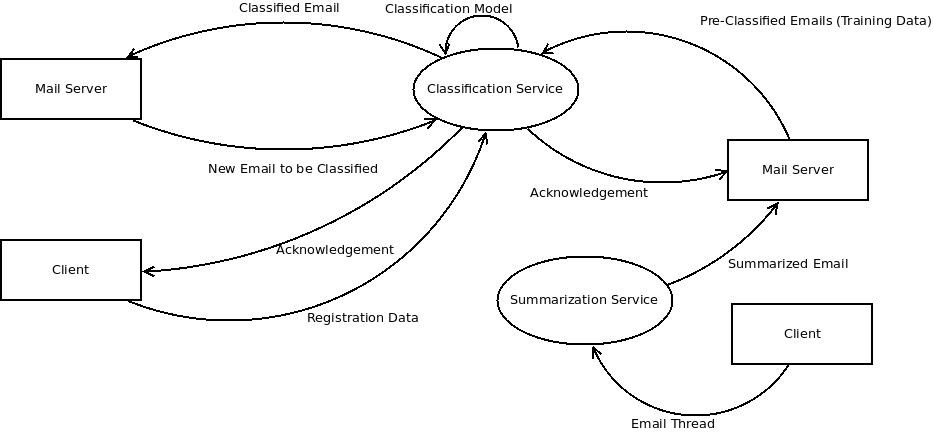
\includegraphics[width=13cm]{context_diagram.jpeg}
%==============================================================================
\subsection{High Level Workflow}
The workflow required to complete the primary objectives of the proposed 
application is described below. The workflow is business-centered, and 
includes ``decision forks'' for decisions the business user, or application, 
must make to achieve the objective. The workflow omits application faults or exceptions. 
Individual tasks in the workflow are described.

\newpage
\begin{my_enumerate}
  \item Workflow/Process Map \\ \\
	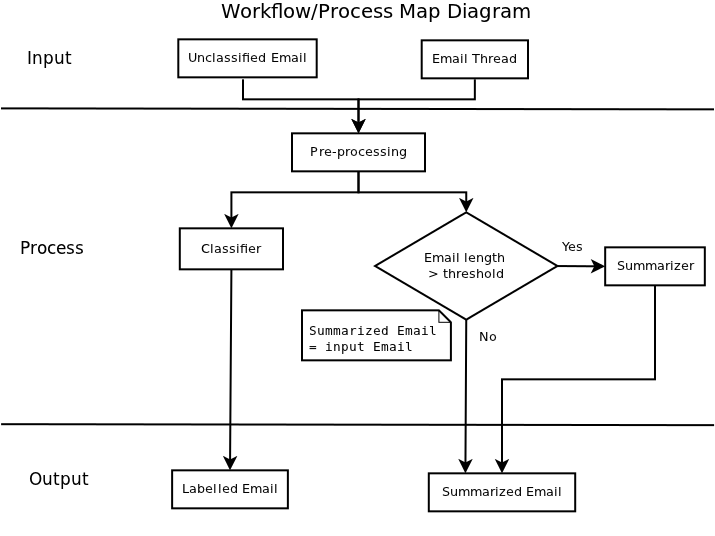
\includegraphics[width=13cm]{workflow_process_map.png}
  \item Workflow Description
  \begin{my_itemize}
    \item Incoming Emails are preprocessed.
    \item Summarization module checks that email length is greater than a predefined threshold:
    \begin{my_itemize}
      \item if the length is greater than the threshold, the email is fed to the 
	    summarizer which outputs the summary;
      \item short emails are returned without summarization.
    \end{my_itemize}
    \item Classification module uses the user model to classify the email into a specific label.
    \item The result is returned by the web service.
  \end{my_itemize}
\end{my_enumerate}

%==============================================================================
\subsection{User stories}
Breaking up the system components to user stories with estimated time (in terms
of man-days = 4 hours) to finish the story is very good practice.
\\

\begin{tabular}{|p{3cm}|p{10cm}|}
\hline
\cellcolor[gray]{0.9} Story Id & \#1 \\ \hline
\cellcolor[gray]{0.9} User Story & Authentication \\ \hline
\cellcolor[gray]{0.9} Priority & Low \\ \hline
\cellcolor[gray]{0.9} Description & 
      As a \textbf{User}, I can \textbf{authenticate the application}. \\ \hline
\cellcolor[gray]{0.9} Estimated time & 1 man-day \\ \hline
\cellcolor[gray]{0.9} Notes & 
      Authentication is done with email username and password. \\ \hline
\end{tabular}

.\\

\begin{tabular}{|p{3cm}|p{10cm}|}
\hline
\cellcolor[gray]{0.9} Story Id & \#2 \\ \hline
\cellcolor[gray]{0.9} User Story & Deauthentication \\ \hline
\cellcolor[gray]{0.9} Priority & Low \\ \hline
\cellcolor[gray]{0.9} Description & 
	As a \textbf{User}, I can \textbf{deauthenticate the application}. \\ \hline
\cellcolor[gray]{0.9} Estimated time & 1 man-day \\ \hline
\cellcolor[gray]{0.9} Notes & 
	Authentication is done with email username and password. \\ \hline
\end{tabular}


.\\

\begin{tabular}{|p{3cm}|p{10cm}|}
\hline
\cellcolor[gray]{0.9} Story Id & \#3 \\ \hline
\cellcolor[gray]{0.9} User Story & Label suggestion \\ \hline
\cellcolor[gray]{0.9} Priority & Medium\\ \hline
\cellcolor[gray]{0.9} Description & 
	As a \textbf{User}, I can \textbf{give feedback for the chosen/suggested labels} to
	\textbf{enhance the classification accuracy}. \\ \hline
\cellcolor[gray]{0.9} Estimated time & 5 man-days\\ \hline
\cellcolor[gray]{0.9} Notes & 
	Build browser extension to support suggestions in gmail. \\ \hline
\end{tabular}

.\\

\begin{tabular}{|p{3cm}|p{10cm}|}
\hline
\cellcolor[gray]{0.9} Story Id & \#4 \\ \hline
\cellcolor[gray]{0.9} User Story & Email Summarization\\ \hline
\cellcolor[gray]{0.9} Priority & High\\ \hline
\cellcolor[gray]{0.9} Description & 
	As a \textbf{User}, I can \textbf{summarize long emails}. \\ \hline
\cellcolor[gray]{0.9} Estimated time & 20 man-days\\ \hline
\cellcolor[gray]{0.9} Notes & 
	The summary will be presented in UI integrated with the email client. \\ \hline
\end{tabular}


.\\

\begin{tabular}{|p{3cm}|p{10cm}|}
\hline
\cellcolor[gray]{0.9} Story Id & \#5 \\ \hline
\cellcolor[gray]{0.9} User Story & Data pre-processing \\ \hline
\cellcolor[gray]{0.9} Priority & High\\ \hline
\cellcolor[gray]{0.9} Description & 
	As a \textbf{System}, I can \textbf{preprocess the dataset} to
	\textbf{make it ready for the classification/summarization process}. \\ \hline
\cellcolor[gray]{0.9} Estimated time & 4 man-days\\ \hline
\cellcolor[gray]{0.9} Notes & 
	Preprocessing includes stemming, checking email length/language,
	removing stop words and identifying the features. \\ \hline
\end{tabular}


.\\

\begin{tabular}{|p{3cm}|p{10cm}|}
\hline
\cellcolor[gray]{0.9} Story Id & \#6 \\ \hline
\cellcolor[gray]{0.9} User Story & Email Classification \\ \hline
\cellcolor[gray]{0.9} Priority & High\\ \hline
\cellcolor[gray]{0.9} Description & 
	As a \textbf{System}, I can \textbf{make online classification to
	an incoming email}. \\ \hline
\cellcolor[gray]{0.9} Estimated time & 20 man-days\\ \hline
\cellcolor[gray]{0.9} Notes & 
	More than one algorithm will be implemented to choose the one with 
	the best accuracy. \\ \hline
\end{tabular}


.\\

\begin{tabular}{|p{3cm}|p{10cm}|}
\hline
\cellcolor[gray]{0.9} Story Id & \#7 \\ \hline
\cellcolor[gray]{0.9} User Story & User Classification Model \\ \hline
\cellcolor[gray]{0.9} Priority & High\\ \hline
\cellcolor[gray]{0.9} Description & 
	As a \textbf{System}, I can \textbf{build a user classification 
	model from the training data}. \\ \hline
\cellcolor[gray]{0.9} Estimated time & 5 man-days\\ \hline
\cellcolor[gray]{0.9} Notes & 
	It will start after user authentication, and can be applied 
	from time to time to enhance the user model. \\ \hline
\end{tabular}

.\\

\begin{tabular}{|p{3cm}|p{10cm}|}
\hline
\cellcolor[gray]{0.9} Story Id & \#8 \\ \hline
\cellcolor[gray]{0.9} User Story & Classification Accuracy test \\ \hline
\cellcolor[gray]{0.9} Priority & Medium \\ \hline
\cellcolor[gray]{0.9} Description & 
	As an \textbf{Admin}, I can \textbf{test the accuracy of the 
	classification algorithm at runtime}. \\ \hline
\cellcolor[gray]{0.9} Estimated time & 2 man-days\\ \hline
\cellcolor[gray]{0.9} Notes & 
	The admin can view the accuracy of the used classification algorithm. \\ \hline
\end{tabular}

.\\

\begin{tabular}{|p{3cm}|p{10cm}|}
\hline
\cellcolor[gray]{0.9} Story Id & \#9 \\ \hline
\cellcolor[gray]{0.9} User Story & Admin Algorithms Control \\ \hline
\cellcolor[gray]{0.9} Priority & Medium \\ \hline
\cellcolor[gray]{0.9} Description & 
	As an \textbf{Admin}, I can \textbf{change/tune the 
	classification/summarization algorithms} to
	\textbf{improve the accuracy}. \\ \hline
\cellcolor[gray]{0.9} Estimated time & 2 man-days\\ \hline
\cellcolor[gray]{0.9} Notes & --- \\ \hline
\end{tabular}

.\\

\begin{tabular}{|p{3cm}|p{10cm}|}
\hline
\cellcolor[gray]{0.9} Story Id & \#10 \\ \hline
\cellcolor[gray]{0.9} User Story & Security \\ \hline
\cellcolor[gray]{0.9} Priority & Medium \\ \hline
\cellcolor[gray]{0.9} Description & 
	As a \textbf{System}, I have to \textbf{ensure a 
	secure connection between the web-service and the email client}. \\ \hline
\cellcolor[gray]{0.9} Estimated time & 1 man-days\\ \hline
\cellcolor[gray]{0.9} Notes & --- \\ \hline
\end{tabular}

%==============================================================================
\newpage
\section{Business Requirements}

This section identifies, enumerates and explores the business requirements that must 
be met by the application. Business requirements include capturing the types of users, 
the basic inputs and outputs, the system's dependencies, and the tasks the system should 
accomplish. It is important to confirm that Task Requirements include all the tasks 
required to meet the business objectives.

%==============================================================================
\subsection{Users}
All applications have users and most have several users of different types. This 
section identifies, at a high level, the types of users of the system.

\begin{my_enumerate}
  \item Application User: requests emails' classification and summarization.
  \item Admin: tunes classification and summarization algorithms and observes the results.
\end{my_enumerate}

%==============================================================================
\subsection{Inputs/Outputs}
This section identifies and describes the inputs to and outputs from the new 
application. Inputs can include electronic inputs, like RSS and EDI feeds, 
updates from external databases, etc, as well as human inputs, like 
``user X keys in results from report Y.'' Output can include electronic feeds, 
printed reports, ...etc. In this section, all electronic inputs and outputs 
are captured. Human inputs are omitted from this section.

\begin{my_enumerate}
  \item Inputs:
  \begin{my_itemize}
    \item unclassified Emails;
    \item classified Emails (training data);
    \item email Threads.
  \end{my_itemize}
  \item Outputs:
  \begin{my_itemize}
    \item classified emails;
    \item summarized email threads;
    \item classification model.
  \end{my_itemize}
\end{my_enumerate}


%==============================================================================
\subsection{Dependencies}
Human inputs are also categorized as dependencies. List all dependencies.

\begin{my_enumerate}
  \item Registeration data.
  \item Request for summarizing an email thread.
\end{my_enumerate}


%==============================================================================
\subsection{Security Requirements}
This section documents, at a high level, the basic security requirements of the 
application. For example, does the system require the user to log in?  Should the 
user’s identity be authenticated on just this system, or against a central authority?  
Are there any special or unusual security requirements, like fingerprint scanning?

\begin{my_enumerate}
  \item The system requires every user to log in with a unique identity (email).
  \item User Data (email) should be transmitted through a secure connection.
  \item Administrators shouldn’t have access to user data (email).
\end{my_enumerate}



%==============================================================================
\subsection{Performance Requirements}
Performance Requirements for the application are defined at a high level below. 
If there are specific requirements for specific features to perform at a quantifiable 
level, they too are listed below. These requirements will be developed in more detail when 
the Requirements Specification is written, in a later phase.

\begin{my_enumerate}
  \item Web service should respond within a reasonable time.
  \item Initial training phase should finish within a reasonable time.
  \item The system will achieve high uptime.
\end{my_enumerate}


%==============================================================================
\subsection{Data Migration}
Data Migration describes the data that needs to be moved from an older or external 
system to the new system, in order for it to operate at launch. Migration also includes 
data that must be transferred from the new system to another external system. 
Any data migration requirements are listed below.

\begin{my_enumerate}
  \item Users' classified emails for training phase as pre-classified emails are needed to build users' models.
  \item Users' email threads which needed to be summarized.
\end{my_enumerate}


\end{document}
